\section{Explain the term symbol (assuming L-S coupling) which describes the state of a multi-electron atom. Use an alkali atom to give an example.}
\sectionmark{Termsymbolet}

\noindent
\large
Termsymbolet antager, at der er LS-kobling
\begin{itemize}
    \item Det regime i finstrukturen, som gælder for de lette atomer, hvor $L$ og $S$ er gode kvantetal, mens jj-koblingen\footnote{jj-koblingen: En enkelt elektrons baneimpulsmoment og spin kobler stærkere med hinanden end hvert af impulsmomenterne gør elektronerne imellem, så $\Vec{J} = \sum_i \Vec{j}_i$, hvor $\Vec{j}_i = \Vec{l}_i + \Vec{s}_i$.} dominerer for tungere atomer, hvor $L$ og $S$ er dårlige kvantetal, da de ikke er entydige -- kun $J$ kan måles
    \item Baneimpulsmomenter $\Vec{L}$ og spin $\Vec{S}$ kobler stærkere indbyrdes end med hinanden, så $\Vec{J} = \Vec{L} + \Vec{S}$, hvor $\Vec{L} = \sum_i \Vec{l}_i$ og $\Vec{S} = \sum_i \Vec{s}_i$
\end{itemize}
Termsymbolet: $n^{2S+1}L_J$
\begin{itemize}
    \item $n$, $S$ og $J$ er de respektive tal, mens $L$ beskriver orbitalen med de nedenstående bogstaver:\\
    \begin{tabular}{|c|c|c|c|c|c|c|}
        \hline
        $L$ & 0 & 1 & 2 & 3 & 4,\: 5,\: \ldots\\
        \hline
        \textbf{Orbital} & S & P & D & F & ''alfabetisk u. J'' \\
        \hline
        \textbf{Navn} & Sharp & Principal & Diffuse & Fundamental & \\
        \hline
    \end{tabular}
\end{itemize}
Hydrogen: $1^2\text{s}_{1/2}$\\
Natrium: $3^2\text{S}_{1/2}$\\
Termsymbol for alkalier generelt: $n^2\text{S}_{1/2}$, hvor $n$ ændres fra atom til atom.\\
Alkalimetaller er ''simple'', da de er hydrogenlignende
\begin{itemize}
    \item Én valenselektron i yderste skal og de indre skaller er helt fyldt
    \begin{itemize}
        \item Dette er dog ikke helt sandfærdigt for alkalimetaller fra $4\text{s}$-orbitalen grundet kvantedefekten i centralfeltsapproksimationen ($4\text{s}$ fyldes før $3\text{p}$, da førstnævnte ligger lavere i energi end sidstnævnte.)
    \end{itemize}
    \item Man kan se et alkalimetal som værende ''hydrogen'' med en større afstand mellem elektron og kerne, samt en kerne med en effektiv kerneladning grundet Gauss' lov:\\
    
    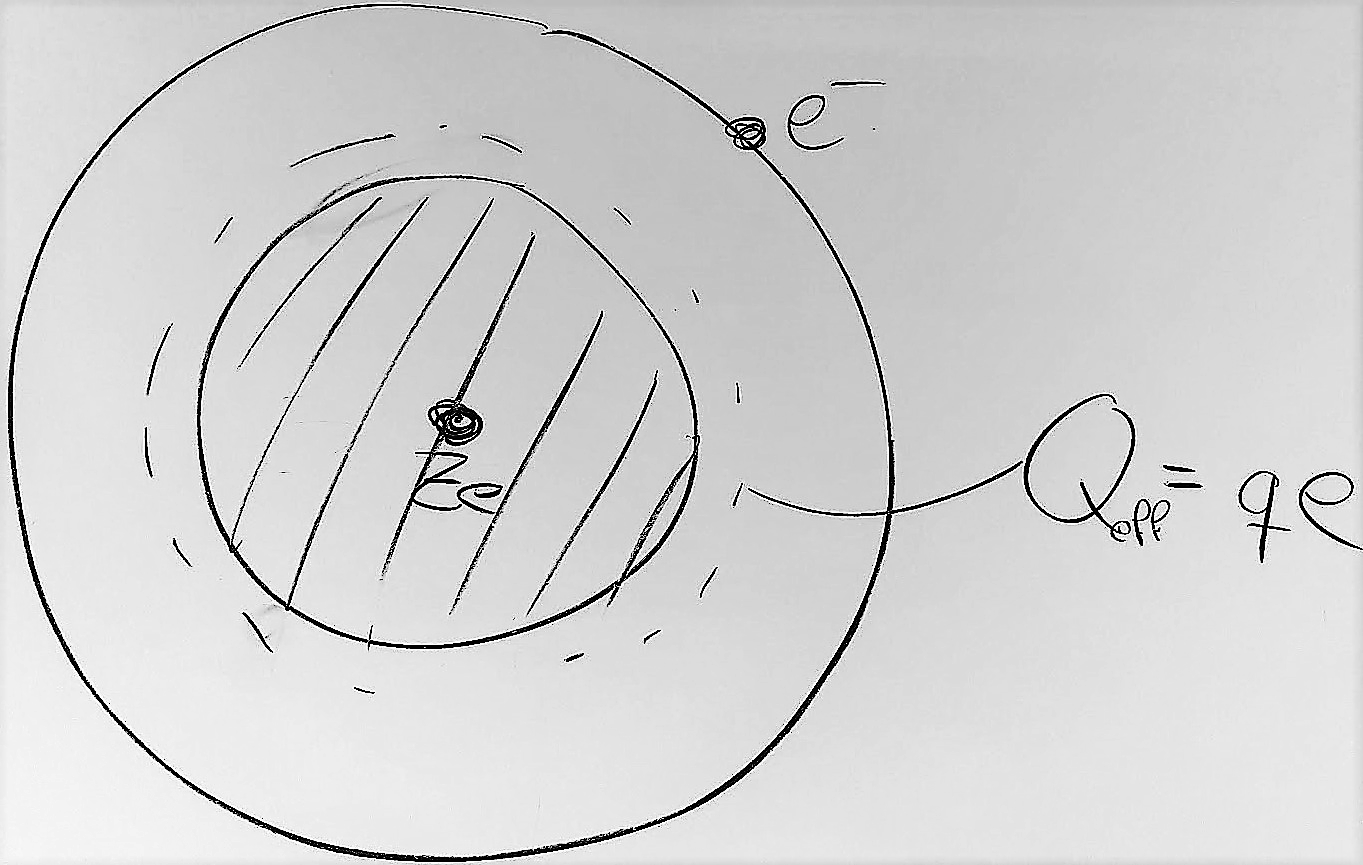
\includegraphics[width=.8\textwidth]{Q14/images/AlkaliSomHydrogenMedEffektivKerneladning.png}
    \item Med variationsregning vil man da (som med heliums grundtilstand) lade den effektive kerneladning være en variabel, som man bruger til at minimere energien (for at finde bølgeunktionen for grundtilstanden), da det altid gør sig gældende, at $E~\ge~E_\text{groundstate}$.
\end{itemize}
\normalsize